\documentclass[twoside,12pt]{article}

\usepackage{dsctemplate}
\usepackage[margin=1in]{geometry}
\usepackage{amsmath}
\usepackage{amssymb,amsthm}
\usepackage{fancyhdr}
\usepackage{nicefrac}
\usepackage{minted}
\usetikzlibrary{quotes,angles,positioning,arrows.meta}
\usetikzlibrary{calc}
\usepackage{enumitem}
\usepackage{fancyvrb}
\usepackage{dirtytalk}
\usepackage{comment}

\DefineVerbatimEnvironment{verbatim}{Verbatim}{xleftmargin=.5in}

% \renewcommand{\rmdefault}{phv} % Arial
% \renewcommand{\sfdefault}{phv} % Arial

% configuration
% ------------------------------------------------------------------------------

% control whether solutions are shown or hidden
\showsolntrue

% page headers only on odd pages
\pagestyle{fancy}
\fancyhead{}
\fancyhead[RO]{PID: \rule{3in}{.5pt}}
\renewcommand{\headrulewidth}{0pt}

% ------------------------------------------------------------------------------

\begin{document}


\thispagestyle{empty}

\vspace{-.5in}

\pstitle{%
    Final Exam%
}{DSC 10, Winter 2023}

\vspace{-.3in}

%\hline

\vspace{.1in}

\textbf{Instructions:}
    \begin{itemize}
        \item This exam consists of 16 questions, worth a total of 164 points.
        \item Write your PID in the top right corner of each page in the space provided.
        \item Please write \textbf{clearly} in the provided answer boxes; we will not grade work that appears elsewhere. Completely fill in bubbles and square boxes; if we cannot tell which option(s) you selected, you may lose points.
        
            ( ) A bubble means that you should only \textbf{select one choice}.
            
            [ ] A square box means you should \textbf{select all that apply}.
        \item Solve all problems using \textbf{the methods of this course}.
        \item You may refer to the Reference Sheet that was provided to you. No calculators, computers, notes, or other aids may be used.
    \end{itemize}
    
\vspace{.1in}

%\hline

\vspace{.1in}

\begin{tabular}{rl}
    Full Name: & \inlineresponsebox[4in]{Solutions}\vspace{.1in}\\
    PID: & \inlineresponsebox[4in]{A12345678}\vspace{.1in}\\
%    Exam start time: & ( ) 9AM} \bubble{10AM} \bubble{11AM} \vspace{.1in\\
%    Initials of student to your left: & \inlineresponsebox[1.5in]{}\\ Initials of student to your right: & \inlineresponsebox[1.5in]{} 
    Seat you are in: & \inlineresponsebox[4in]{}\
\end{tabular}

\vspace{.25in}

\noindent By signing below, you are agreeing that you will behave honestly and fairly during
and after this exam.

\begin{tabular}{rl}
    \: \: \: \: \: Signature: & \inlineresponsebox[4in]{}\\
\end{tabular}

\vfill

\begin{center}
{\huge Version A} \vspace{.2in}
\end{center}

\noindent \textbf{Please do not open your exam until instructed to do so, but you may read the data description attached to the Reference Sheet.}

\vspace{1em}


\newpage

\noindent \textbf{Make sure you have read the data description attached to the Reference Sheet!}

\vspace{0.2in}



# BEGIN PROB



Let's start by correcting the data in the \texttt{"Rating"} column. All the values in this column are strings of length 4. In addition, some strings use commas in place of a dot to represent a decimal point. Select the options below that evaluate to a Series containing the values in the \texttt{"Rating"} column, appropriately changed to floats.

\textbf{Note:} The Series method \texttt{.str.replace} uses the string method \texttt{.replace} on every string in a Series. 

\vspace{0.1in}

[ ] \texttt{float(games.get("Rating").str.replace(",", "."))}

[ ] \texttt{games.get("Rating").str.replace(",", ".").apply(float)}

[ ] \texttt{games.get("Rating").str.replace(",", "").apply(int)/100}

[ ] \texttt{games.get("Rating").str.replace(",", "").apply(float)}

\vspace{0.1in}

\textbf{Important!} For the rest of this exam, we will assume that the values in the \texttt{"Rating"} column have been correctly changed to floats. 



# END PROB

\vspace{0.5in}

# BEGIN PROB



You are unsure whether it would make sense to use \texttt{"BGG Rank"} as the index of the \texttt{games} DataFrame, because you are unsure whether this column can have duplicate values. Perhaps, for example, two games are tied and both have a rank of 6. 

Select all of the expressions below that evaluate to True when the\texttt{"BGG Rank"} column could be used as the index (no duplicates), and False when it could not be used as the index (duplicates). In other words, these are the expressions that can be used to detect the presence of duplicate values.

\vspace{0.1in}

[ ] \texttt{(games.get("BGG Rank") - np.arange(games.shape[0])).max() == 1}

[ ] \texttt{games.groupby("BGG Rank").count().get("Name").max() == 1}

[ ] \texttt{games.shape[0] - len(np.unique(games.get("BGG Rank"))) == 0}

[ ] \texttt{games.get("BGG Rank").max() - games.shape[0] == 0}

\vspace{0.1in}

\textbf{Note:} We will not set the index of \texttt{games}, instead we'll leave it with the default index.


# END PROB

\newpage
# BEGIN PROB

[(14 pts)]

        Notice that \texttt{"Strategy Games"} and \texttt{"Thematic Games"} are two of the possible domains, and that a game can belong to multiple domains. 

        Define the variables \texttt{strategy} and \texttt{thematic} follows.

\begin{verbatim}
strategy = games.get("Domains").str.contains("Strategy Games")
thematic = games.get("Domains").str.contains("Thematic Games")
\end{verbatim}


    # BEGIN SUBPROB


        What is the data type of \texttt{strategy}?

        \begin{center}
            ( ) \texttt{bool} 
            ( ) \texttt{str} 
            ( ) \texttt{Series} 
            ( ) \texttt{DataFrame} 
        \end{center}

    

# END SUBPROB

    # BEGIN SUBPROB


        
        Suppose we randomly select one of the \texttt{"Strategy Games"} from the \texttt{games} DataFrame. What is the probability that the randomly selected game is \textbf{not} also one of the \texttt{"Thematic Games"}? In the space below, write a single line of Python code that evaluates to this probability, using the variables \texttt{strategy} and \texttt{thematic} in your solution.

        \textbf{Note:} For this question and others that require one line of code, it's fine if you need to write your solution on multiple lines, as long as it is just one line of Python code. Please do write on multiple lines to make sure your answer fits within the box provided.

        \begin{responsebox}{2in}

            Here are two possible answers:
            
\texttt{(games[(strategy == True) \& (thematic == False)].shape[0]}\\
\texttt{/ games[strategy == True].shape[0])}    

\texttt{1 - games[strategy \& thematic].shape[0] / games[strategy].shape[0]}
           
        \end{responsebox}
        
    

# END SUBPROB
    # BEGIN SUBPROB


        Many of the games in the \texttt{games} DataFrame belong to more than one domain. We want to identify the number of games that belong to only one domain. Select all of the options below that would correctly calculate the number of games that belong to only one domain. 

        \textbf{Hint:} Don't make any assumptions about the possible domains.

        \vspace{0.1in}

        [ ] \texttt{(games.get("Domains").str.split(" ").apply(len) == 2).sum()}

        [ ] \texttt{(games.get("Domains").apply(len) == 1).sum()}

        \correctsquarebubble{\texttt{(games[games.get("Domains").str.split(",").apply(len) == 1]\\
        \hspace*{1em}.groupby("Domains").count().get("Name").sum())}}

        [ ] \texttt{games[games.get("Domains").str.split(",").apply(len) == 1].shape[0]}
    

# END SUBPROB




# END PROB

\newpage
# BEGIN PROB



We want to create a bootstrapped 95\% confidence interval for the median \texttt{"Complexity"} of all cooperative games, given a sample of 100 cooperative games. 

Suppose \texttt{coop\_sample} is a DataFrame containing 100 rows of \texttt{games}, all of which are cooperative games. We'll calculate the endpoints \texttt{left} and \texttt{right} of our bootstrapped 95\% confidence interval as follows.

\begin{verbatim}
medians = np.array([])
for i in np.arange(10000):
    resample = coop_sample.sample(100, replace=True)
    median = np.median(resample.get("Complexity"))
    medians = np.append(medians, median)
left = np.percentile(medians, 2.5)
right = np.percentile(medians, 97.5)
\end{verbatim}


    # BEGIN SUBPROB


        Now consider the interval defined by the endpoints \texttt{left\_2} and \texttt{right\_2}, calculated as follows. 

\begin{verbatim}
medians_2 = np.array([])
for i in np.arange(10000):
    shuffle = coop_sample.assign(shuffle=
              np.random.permutation(coop_sample.get("Complexity")))
    resample_2 = shuffle.sample(100, replace=True)
    median_2 = np.median(resample_2.get("shuffle"))
    medians_2 = np.append(medians_2, median_2)
left_2 = np.percentile(medians_2, 2.5)
right_2 = np.percentile(medians_2, 97.5)
\end{verbatim}

        Which interval should be wider, \texttt{[left, right]} or \texttt{[left\_2, right\_2]}?

        \begin{center}
            ( ) \texttt{[left, right]} 
             ( ) \texttt{[left\_2, right\_2]} 
            ( ) Both about the same.
        \end{center}
        
    

# END SUBPROB
    # BEGIN SUBPROB


        Now consider the interval defined by the endpoints \texttt{left\_3} and \texttt{right\_3}, calculated as follows. 

\begin{verbatim}
medians_3 = np.array([])
for i in np.arange(10000):
    resample_3 = (coop_sample.sample(100, replace=True)
                             .sample(100, replace=True))
    median_3 = np.median(resample_3.get("Complexity"))
    medians_3 = np.append(medians_3, median_3)
left_3 = np.percentile(medians_3, 2.5)
right_3 = np.percentile(medians_3, 97.5)
\end{verbatim}

        Which interval should be wider, \texttt{[left, right]} or \texttt{[left\_3, right\_3]}?

        \begin{center}
            ( ) \texttt{[left, right]} 
             ( ) \texttt{[left\_3, right\_3]} 
            ( ) Both about the same.
        \end{center}
              
    

# END SUBPROB



# END PROB

\newpage
# BEGIN PROB

[(12 pts)]

As in the previous question, let \texttt{coop\_sample} be a sample of 100 rows of \texttt{games}, all corresponding to cooperative games.

Define \texttt{samp} and \texttt{resamp} as follows.

\begin{verbatim}
samp = coop_sample.get("Complexity")
resamp = coop_sample.sample(100, replace=True).get("Complexity")
\end{verbatim}


    # BEGIN SUBPROB


        Which of the following statements \textbf{could} evaluate to \texttt{True}? Select all that are possible.

        \vspace{0.1in}

            [ ] \texttt{len(samp.unique()) < len(resamp.unique())}} \hspace{0.5in
            
            [ ] \texttt{len(samp.unique()) ==  len(resamp.unique())}} \hspace{0.5in
            
            [ ] \texttt{len(samp.unique()) > len(resamp.unique())}

        
    

# END SUBPROB
        # BEGIN SUBPROB


        Which of the following statements \textbf{could} evaluate to \texttt{True}? Select all that are possible.

        \vspace{0.1in}

            [ ] \texttt{np.count\_nonzero(samp == 1) < np.count\_nonzero(resamp == 1)}
            
            [ ] \texttt{np.count\_nonzero(samp == 1) == np.count\_nonzero(resamp == 1)}
            
            [ ] \texttt{np.count\_nonzero(samp == 1) > np.count\_nonzero(resamp == 1)}

        
    

# END SUBPROB
        # BEGIN SUBPROB


        Which of the following statements \textbf{could} evaluate to \texttt{True}? Select all that are possible.

        \vspace{0.1in}

            [ ] \texttt{samp.min() < resamp.min()}
            
            [ ] \texttt{samp.min() == resamp.min()}
            
            [ ] \texttt{samp.min() > resamp.min()}

        
    

# END SUBPROB
        # BEGIN SUBPROB


        Which of the following statements \textbf{could} evaluate to \texttt{True}? Select all that are possible.

        \vspace{0.1in}

            [ ] \texttt{np.std(samp) < np.std(resamp)}
            
            [ ] \texttt{np.std(samp) == np.std(resamp)}
            
            [ ] \texttt{np.std(samp) > np.std(resamp)}
   
    

# END SUBPROB




# END PROB

\newpage
# BEGIN PROB



Choose the best tool to answer each of the following questions. Note the following:
\begin{itemize}
    \item By ``hypothesis testing," we mean ``standard" hypothesis testing, i.e. hypothesis testing that \textbf{doesn't} involve permutation testing or bootstrapping.
    \item By ``bootstrapping," we mean bootstrapping that \textbf{doesn't} involve hypothesis testing.
\end{itemize}


    # BEGIN SUBPROB


        Are strategy games rated higher than non-strategy games?

        \begin{center}
            ( ) Hypothesis testing
            ( ) Permutation testing
            ( ) Bootstrapping           
        \end{center}

    

# END SUBPROB
    # BEGIN SUBPROB


        What is the mean complexity of all games?

        \begin{center}
            ( ) Hypothesis testing
            ( ) Permutation testing
            ( ) Bootstrapping           
        \end{center}
        
    

# END SUBPROB
    # BEGIN SUBPROB


        Are there an equal number of cooperative and non-cooperative games?

        \begin{center}
            ( ) Hypothesis testing
            ( ) Permutation testing
            ( ) Bootstrapping           
        \end{center}
        
    

# END SUBPROB
    # BEGIN SUBPROB


        Are games with more than one domain more complex than games with one domain?

        \begin{center}
            ( ) Hypothesis testing
            ( ) Permutation testing
            ( ) Bootstrapping           
        \end{center}
        
    

# END SUBPROB




# END PROB

\newpage
# BEGIN PROB



We use the regression line to predict a game's \texttt{"Rating"} based on its \texttt{"Complexity"}. We find that for the game \textit{Wingspan}, which has a \texttt{"Complexity"} that is 2 points higher than the average, the predicted \texttt{"Rating"} is 3 points higher than the average. 


    # BEGIN SUBPROB

 What can you conclude about the correlation coefficient $r$?

     \vspace{0.1in}
     
        ( ) $r < 0$
             
        ( ) $r = 0$
        
        ( ) $r > 0$
              
        \bubble{We cannot make any conclusions about the value of $r$ based on this information\\
        \hspace*{1em} alone.}
    

# END SUBPROB
    # BEGIN SUBPROB

 What can you conclude about the standard deviations of \texttt{"Complexity"} and \texttt{"Rating"}?

         \vspace{0.1in}
    
        ( ) SD of \texttt{"Complexity"} $<$ SD of \texttt{"Rating"}
        
        ( ) SD of \texttt{"Complexity"} $=$ SD of \texttt{"Rating"}
        
        ( ) SD of \texttt{"Complexity"} $>$ SD of \texttt{"Rating"}
        
        \bubble{We cannot make any conclusions about the relationship between these two standard\\
        \hspace*{1em} deviations based on this information alone.}
    

# END SUBPROB




# END PROB

\vspace{0.5in}

# BEGIN PROB



Suppose that for children's games, \texttt{"Play Time"} and \texttt{"Rating"} are negatively linearly associated due to children having short attention spans. Suppose that for children's games, the standard deviation of \texttt{"Play Time"} is twice the standard deviation of \texttt{"Rating"}, and the average \texttt{"Play Time"} is 10 minutes. 

We use linear regression to predict the \texttt{"Rating"} of a children's game based on its \texttt{"Play Time"}. The regression line predicts that \textit{Don't Break the Ice}, a children's game with a \texttt{"Play Time"} of 8 minutes will have a \texttt{"Rating"} of 4. Which of the following could be the average \texttt{"Rating"} for children's games?

        \begin{center}
            ( ) $2$}    \hspace{0.5in
            ( ) $2.8$}   \hspace{0.5in  
            ( ) $3.1$}   \hspace{0.5in       
            ( ) $4$ 
        \end{center}



# END PROB

\newpage
# BEGIN PROB

[(15 pts)]

The function \texttt{perm\_test} should take three inputs:

\begin{enumerate}
    \item \texttt{df}, a DataFrame.
    \item \texttt{labels}, a string. The name of a column in \texttt{df} that contains two distinct values, which signify the groups in a permutation test.
    \item \texttt{data}, a string. The name of a column in \texttt{df} that contains numerical data. 
\end{enumerate}

The function should return an array of 1000 simulated differences of group means, under the assumption of the null hypothesis in a permutation test, namely that data in both groups come from the same population. 

The smaller of the two group labels should be first in the subtraction. For example, if the two values in the \texttt{labels} column are \texttt{"dice game"} and \texttt{"card game"}, we would compute the difference as the mean of the \texttt{"card game"} group minus the mean of the \texttt{"dice game"} group, because \texttt{"card game"} comes before \texttt{"dice game"} alphabetically. Note that \textbf{groupby} orders the rows in ascending order by default.

        An incorrect implementation of \texttt{perm\_test} is provided below. 
    
\begin{verbatim}[numbers=left]
def perm_test(df, labels, data):
    diffs = np.array([])
    for i in np.arange(1000):
        df.assign(shuffled=np.random.permutation(df.get(data)))  
        means = df.groupby(labels).mean().get(data)
        diff = means.iloc[0] - means.iloc[1]
        diffs = np.append(diffs, diff)
        return diffs
\end{verbatim}

Three lines of code above are incorrect. Your job is to identify which lines of code are incorrect, and describe briefly in English how you would fix them. You don't need to explain why the current code is wrong, just how to fix it.

\newpage
    
        
            # BEGIN SUBPROB

    
                The first line that is incorrect is line number \inlineresponsebox[0.5in]{4}.
            
                Explain in one sentence how to change this line. Do not write code.
                \begin{responsebox}{1.5in}
                    We need to save this as \texttt{df}.
                \end{responsebox}
            

# END SUBPROB
            # BEGIN SUBPROB

    
                The second line that is incorrect is line number \inlineresponsebox[0.5in]{5}.
            
                Explain in one sentence how to change this line. Do not write code.
                \begin{responsebox}{1.5in}
                    We need to get \texttt{"shuffled"} instead of \texttt{data}.
                \end{responsebox}
            

# END SUBPROB
            # BEGIN SUBPROB

    
                The third line that is incorrect is line number \inlineresponsebox[0.5in]{8}.
            
                Explain in one sentence how to change this line. Do not write code.
                \begin{responsebox}{1.5in}
                    Move it outside of the \texttt{for} loop (unindent).
                \end{responsebox}
            

# END SUBPROB
            

\newpage 

        Suppose you've fixed all the issues with this function, as you described above. Now, you want to use this corrected function to run a permutation test with the following hypotheses:

        \begin{itemize}
            \item \textbf{Null Hypothesis}: The play time of children's dice-rolling games and the play time of children's non-dice-rolling games come from the same distribution.
            \item \textbf{Alternative Hypothesis}: The play time of children's dice-rolling games is lower, on average, than the play time of children's non-dice-rolling games.
        \end{itemize}
        
        
        For this permutation test, consider a children's game to be a game that has \texttt{"Children's Games"} as part of the \texttt{"Domains"} column. A dice-rolling game is one that has \texttt{"Dice Rolling"} as part of the \texttt{"Mechanics"} column, and a non-dice-rolling game is one that does not have \texttt{"Dice Rolling"} as part of the \texttt{"Mechanics"} column.
        
        The DataFrame \texttt{with\_dice} is defined as follows.  

\begin{verbatim}
with_dice = games.assign(isDice = games.get("Mechanics")
                                       .str.contains("Dice Rolling"))
\end{verbatim}
    
    
    # BEGIN SUBPROB


        Write one line of code that creates an array called \texttt{simulated\_diffs} containing 1000 simulated differences in group means for this permutation test. You should call your \texttt{perm\_test} function here!

        \begin{responsebox}{2in}
            \texttt{simulated\_diffs = perm\_test(with\_dice[with\_dice.get("Domains")
            .str.contains("Children's Games")], "isDice", "Play Time")}
        \end{responsebox}
    

# END SUBPROB
    # BEGIN SUBPROB


        Suppose we've stored the observed value of the test statistic for this permutation test in the variable \texttt{obs\_diff}. Fill in the blank below to find the p-value for this permutation test.

\begin{verbatim}
p_value = np.count_nonzero(simulated_diffs ____ obs_diff)/1000
\end{verbatim}

        What goes in the blank? 

        \begin{center}
            ( ) \texttt{<}         
            ( ) \texttt{<=}        
            ( ) \texttt{>}        
            ( ) \texttt{>=}
        \end{center}
        
    

# END SUBPROB




# END PROB

\newpage
# BEGIN PROB



It's your first time playing a new game called \textit{Brunch Menu}. The deck contains 96 cards, and each player will be dealt a hand of 9 cards. The goal of the game is to avoid having certain cards, called \textit{Rotten Egg} cards, which come with a penalty at the end of the game. But you're not sure how many of the 96 cards in the game are \textit{Rotten Egg} cards. So you decide to use the Central Limit Theorem to estimate the proportion of \textit{Rotten Egg} cards in the deck based on the 9 random cards you are dealt in your hand.


    # BEGIN SUBPROB


        You are dealt 3 \textit{Rotten Egg} cards in your hand of 9 cards. You then construct a CLT-based 95\% confidence interval for the proportion of \textit{Rotten Egg} cards in the deck based on this sample. Approximately, how wide is your confidence interval? 

        \vspace{0.1in}

        Choose the closest answer, and use the following facts:
        \begin{itemize}
            \item The standard deviation of a collection of 0s and 1s is
            $$\sqrt{(\text{Prop. of 0s}) \times (\text{Prop. of 1s})}.$$
            \item $\sqrt{18}$ is about $\frac{17}{4}$.
        \end{itemize}

        \begin{center}
        ( ) $\dfrac{17}{9}$}    \hspace{0.5in
        ( ) $\dfrac{17}{27}$}   \hspace{0.5in  
        ( ) $\dfrac{17}{81}$}   \hspace{0.5in       
        ( ) $\dfrac{17}{96}$ 
        \end{center}
    

# END SUBPROB
    # BEGIN SUBPROB


        Which of the following are limitations of trying to use the Central Limit Theorem for this particular application? Select all that apply.

        \vspace{0.1in}

            [ ] The CLT is for large random samples, and our sample was not very large.
            
            \correctsquarebubble{The CLT is for random samples drawn with replacement, and our sample was drawn\\
            \hspace*{1em} without replacement.}
            
            \squarebubble{The CLT is for normally distributed data, and our data may not have been normally\\
            \hspace*{1em} distributed.}
            
            [ ] The CLT is for sample means and sums, not sample proportions.
    

# END SUBPROB



# END PROB

\newpage
# BEGIN PROB



In recent years, there has been an explosion of board games that teach computer programming skills, including \textit{CoderMindz}, \textit{Robot Turtles}, and \textit{Code Monkey Island}. Many such games were made possible by Kickstarter crowdfunding campaigns. 

Suppose that in one such game, players must prove their understanding of functions and conditional statements by answering questions about the function \texttt{wham}, defined below. Like players of this game, you'll also need to answer questions about this function.

\begin{verbatim}[numbers=left]
def wham(a,b):
    if a < b:
        return a + 2
    if a + 2 == b:
        print(a + 3)
        return b + 1
    elif a - 1 > b:
        print(a)
        return a + 2
    else:
        return a + 1
\end{verbatim}


    # BEGIN SUBPROB


        What is printed when we run \texttt{print(wham(6, 4))}?

        \begin{responsebox}{1in}
        
            6 \\
            8
        \end{responsebox}
    

# END SUBPROB
    # BEGIN SUBPROB


        Give an example of a pair of integers \texttt{a} and \texttt{b} such that \texttt{wham(a, b)} returns \texttt{a + 1}.

        \begin{center}
            \texttt{a} = \inlineresponsebox[1in]{4}, \texttt{b} = \inlineresponsebox[1in]{4}            
        \end{center}

        # BEGIN SOLN


        Any pair of integers \texttt{a}, \texttt{b} with \texttt{a = b} or \texttt{a = b + 1} is correct.
        

# END SOLN
        

    

# END SUBPROB
    # BEGIN SUBPROB


        Which of the following lines of code will never be executed, for any input?

        \begin{center}
            ( ) $3$}  \hspace{0.5in      
            ( ) $6$}     \hspace{0.5in   
            ( ) $9$}      \hspace{0.5in   
            ( ) $11$           
        \end{center}

 
    

# END SUBPROB    






# END PROB

\newpage
# BEGIN PROB



In the game \textit{Spot It}, players race to identify an object that appears on two different cards. Each card contains images of eight objects, and exactly one object is common to both cards. 

\vspace*{-0.2in}

\begin{center}
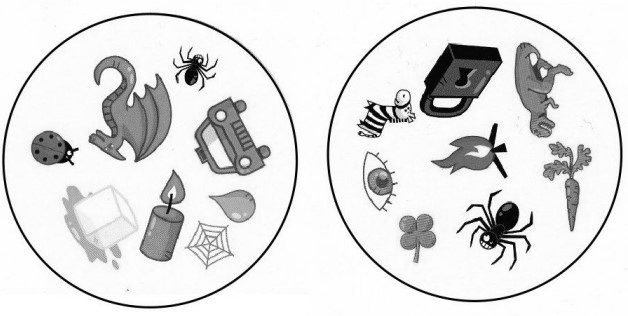
\includegraphics[width=3.5in]{final_images/spot.jpg}
\end{center}

\vspace*{-0.4in}


    # BEGIN SUBPROB


    Suppose the objects appearing on each card are stored in an array, and our task is to find the object that appears on both cards. Complete the function \texttt{find\_match} that takes as input two arrays of 8 objects each, with one object in common, and returns the name of the object in both arrays.

    For example, suppose we have two arrays defined as follows.

\begin{verbatim}
objects1 = np.array(["dragon", "spider", "car", "water droplet", 
                     "spiderweb", "candle", "ice cube", "ladybug"]) 
objects2 = np.array(["zebra", "lock", "dinosaur", "eye", "fire",
                     "shamrock", "spider", "carrot"])
\end{verbatim}

    Then \texttt{find\_match(objects1, objects2)} should evaluate to \texttt{"spider"}.

    Your function must include a \texttt{for} loop, and it must take \textbf{at most three lines of code} (not counting the line with \texttt{def}).

\begin{mdframed}
\begin{verbatim}
def find_match(array1, array2):
    for obj in array1:
        if obj in array2:
            return obj
            
\end{verbatim}
\end{mdframed}
     
        
    

# END SUBPROB
    # BEGIN SUBPROB


        Now suppose the objects appearing on each card are stored in a DataFrame with 8 rows and one column called \texttt{"object"}. Complete the function \texttt{find\_match\_again} that takes as input two such DataFrames with one object in common and returns the name of the object in both DataFrames. 

        Your function may not call the previous function \texttt{find\_match}, and it must take \textbf{exactly one line of code} (not counting the line with \texttt{def}).

\begin{mdframed}
\begin{verbatim}
def find_match_again(df1, df2):
    return df1.merge(df2, on="item").get("item").iloc[0]
    
\end{verbatim}
\end{mdframed}

    

# END SUBPROB




# END PROB

\newpage
# BEGIN PROB

[(16 pts)]

Dylan, Harshi, and Selim are playing a variant of a dice game called \textit{Left, Center, Right (LCR)} in which there are $9$ chips (tokens) and $9$ dice. Each player starts off with $3$ chips. Each die has the following six sides: L, C, R, Dot, Dot, Dot. 

During a given player's turn, they must roll a number of dice equal to the number of chips they currently have. Each die determines what to do with one chip:
\begin{enumerate}
\item L means give the chip to the player on their left.
\item R means give the chip to the player on their right.
\item C means put the chip in the center of the table. This chip is now out of play.
\item Dot means do nothing (or keep the chip).
\end{enumerate}
Since the number of dice rolled is the same as the number of chips the player has, the dice rolls determine exactly what to do with each chip. There is no strategy at all in this simple game.

Dylan will take his turn first (we'll call him Player 0), then at the end of his turn, he'll pass the dice to his left and play will continue clockwise around the table. Harshi (Player 1) will go next, then Selim (Player 2), then back to Dylan, and so on. 

\begin{center}
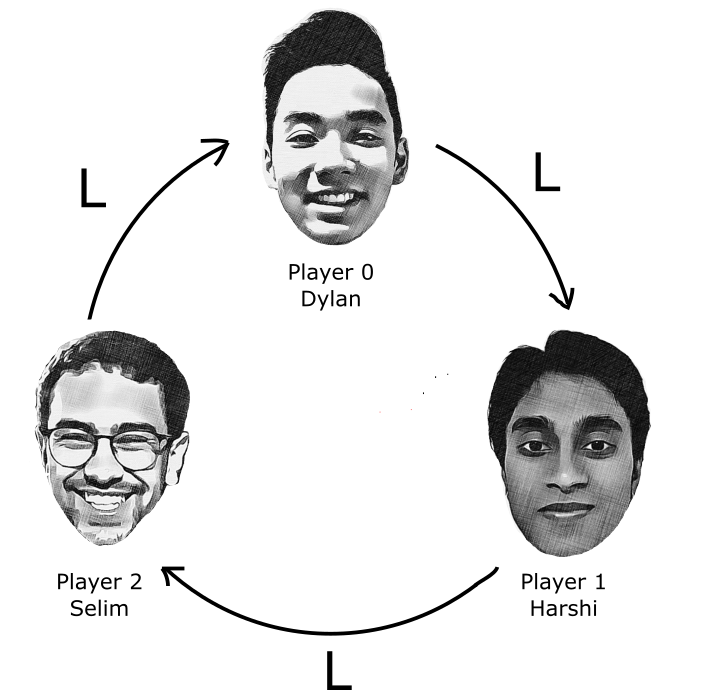
\includegraphics[width=3.5in]{final_images/lcr.png}
\end{center}

Note that if someone has no chips when it's their turn, they are still in the game and they still take their turn, they just roll 0 dice because they have 0 chips.  The game ends when only one person is holding chips, and that person is the winner. If 300 turns have been taken (100 turns each), the game will end and we'll declare it a tie.

\newpage

The function \texttt{simulate\_lcr} below simulates one full game of \textit{Left, Center, Right} and returns the number of turns taken in that game. Some parts of the code are not provided. You will need to fill in the code for the parts marked with a blank. The parts marked with \texttt{...} are not provided, but you don't need to fill them in because they are very similar to other parts that you do need to complete.

\textbf{Hint:} Recall that in Python, the $\%$ operator gives the remainder upon division. For example $12~\%~5$ is $2$.

\begin{verbatim}
def simulate_lcr():
    # stores the number of chips for players 0, 1, 2 (in that order)
    player_chips = np.array([3,3,3]) 
    
    # maximum of 300 turns allotted for the game
    for i in np.arange(300): 
    
        # which player's turn it is currently (0, 1, or 2)
        current_player = __(a)__
    
        # stores what the player rolled on their turn
        roll = np.random.choice(["L", "C", "R", "Dot", "Dot", "Dot"], 
                                __(b)__) 
    
        # count the number of instances of L, C, and R
        L_count = __(c)__
        C_count = ...
        R_count = ...
    
        if current_player == 0:
            # update player_chips based on what player 0 rolled
            player_chips = player_chips + np.array(__(d)__)
        elif current_player == 1:
            # update player_chips based on what player 1 rolled
            player_chips = player_chips + ...
        else:
            # update player_chips based on what player 2 rolled
            player_chips = player_chips + ...
        
        # if the game is over, return the number of turns played
        if __(e)__:
            return __(f)__ 

    # if no one wins after 300 turns, return 300
    return 300
\end{verbatim}

\newpage


    # BEGIN SUBPROB


        What goes in blank (a)?

        \begin{responsebox}{0.5in}
        \texttt{i \% 3} 
        \end{responsebox}
    

# END SUBPROB
    # BEGIN SUBPROB


        What goes in blank (b)?

        \begin{responsebox}{0.5in}
        \texttt{player\_chips[current\_player]}     
        \end{responsebox}
    

# END SUBPROB
    # BEGIN SUBPROB


        What goes in blank (c)?

        \begin{responsebox}{0.5in}
         \texttt{np.count\_nonzero(roll == "L")}    
        \end{responsebox}
    

# END SUBPROB
    # BEGIN SUBPROB


        What goes in blank (d)?

        \begin{responsebox}{0.5in}
         \texttt{[-(L\_count + C\_count + R\_count), L\_count, R\_count]}    
        \end{responsebox}
    

# END SUBPROB
    # BEGIN SUBPROB


        What goes in blank (e)?

        \begin{responsebox}{0.5in}
         \texttt{np.count\_nonzero(player\_chips) == 1}    
        \end{responsebox}
    

# END SUBPROB
    # BEGIN SUBPROB


        What goes in blank (f)?
        
        \begin{responsebox}{0.5in}
           \texttt{i + 1}  
        \end{responsebox}
    

# END SUBPROB




# END PROB

\newpage
# BEGIN PROB

[(14 pts)]

Suppose the function \texttt{simulate\_lcr} from the last question has been correctly implemented, and we want to use it to see how many turns a game of \textit{Left, Center, Right} usually takes. 

\textbf{Note:} You can answer this question even if you couldn't answer the previous one.


    # BEGIN SUBPROB

 Consider the code and histogram below.

\begin{verbatim}
turns = np.array([])
for i in np.arange(10000):
    turns = np.append(turns, simulate_lcr())   
(bpd.DataFrame().assign(turns=turns)
                .plot(kind="hist", density = True, 
                      ec="w", bins = np.arange(0, 66, 6)))
\end{verbatim}

\begin{center}
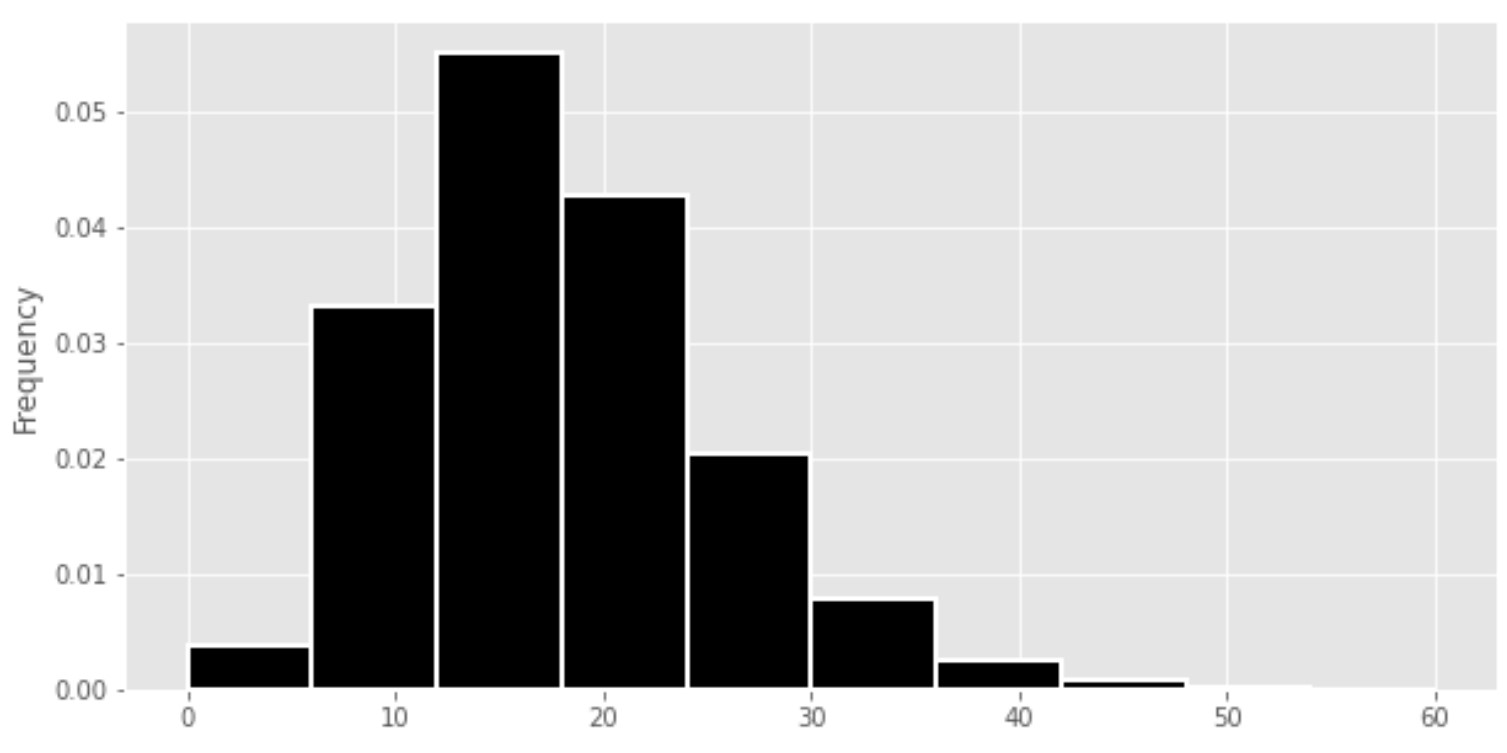
\includegraphics[width=3.5in]{final_images/hist.jpg}
\end{center}

        \begin{enumerate}[label=(\roman*)]
        \item Does this histogram show a probability distribution or an empirical distribution?

        \begin{center}        
            ( ) Probability distribution
            ( ) Empirical distribution
        \end{center}

        \item What is the probability of a game of \textit{Left, Center, Right} lasting 30 turns or more?  Choose the closest answer below.

        \begin{center}
            ( ) 0.01        
            ( ) 0.06        
            ( ) 0.10        
            ( ) 0.60
        \end{center}
        
        \end{enumerate}
    

# END SUBPROB
    # BEGIN SUBPROB


        Suppose a player with $n$ chips takes their turn. What is the probability that they will have to put at least one chip into the center? Give your answer as a mathematical expression involving $n$.
        \begin{responsebox}{0.5in}
            $1 - \left(\frac{5}{6}\right)^n$
        \end{responsebox}
    

# END SUBPROB
    # BEGIN SUBPROB


        Suppose a player with n chips takes their turn. What is the probability that they will end their turn with $n$ chips? Give your answer as a mathematical expression involving $n$.
        \begin{responsebox}{0.5in}
            $\left(\frac{1}{2}\right)^n$
        \end{responsebox}
    

# END SUBPROB





# END PROB

\newpage
# BEGIN PROB

[(12 pts)]

At a recent game night, you played several new board games and liked them so much that you now want to buy copies for yourself. 

The DataFrame \texttt{stores} is shown below in full. Each row represents a game you want to buy and a local board game store where that game is available for purchase. If a game is not available at a certain store, there will be no row corresponding to that store and that game.

\begin{center}
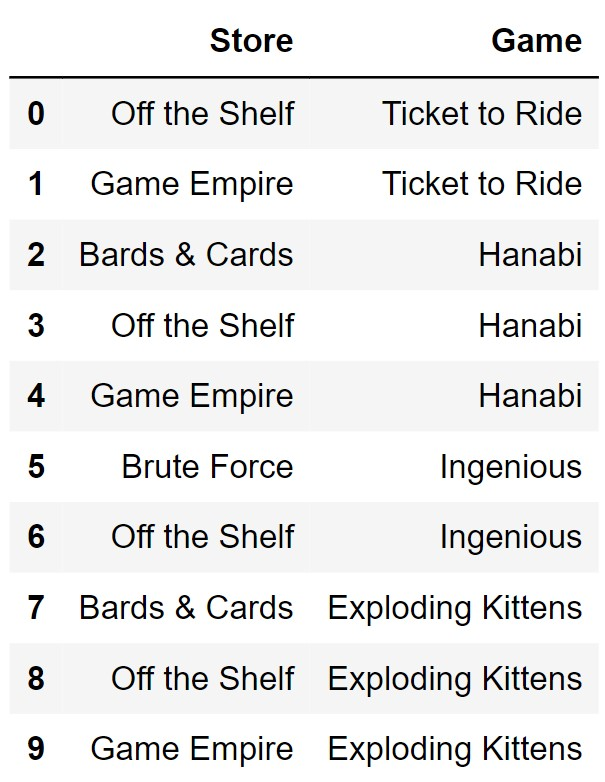
\includegraphics[width=2in]{final_images/stores.jpg}
\end{center}


    # BEGIN SUBPROB


        The DataFrame \texttt{prices} has \textbf{five rows}. Below we merge \texttt{stores} with \texttt{prices} and display the output in full.

\begin{verbatim}
merged = stores.merge(prices, on="Game")
merged
\end{verbatim}

\begin{center}
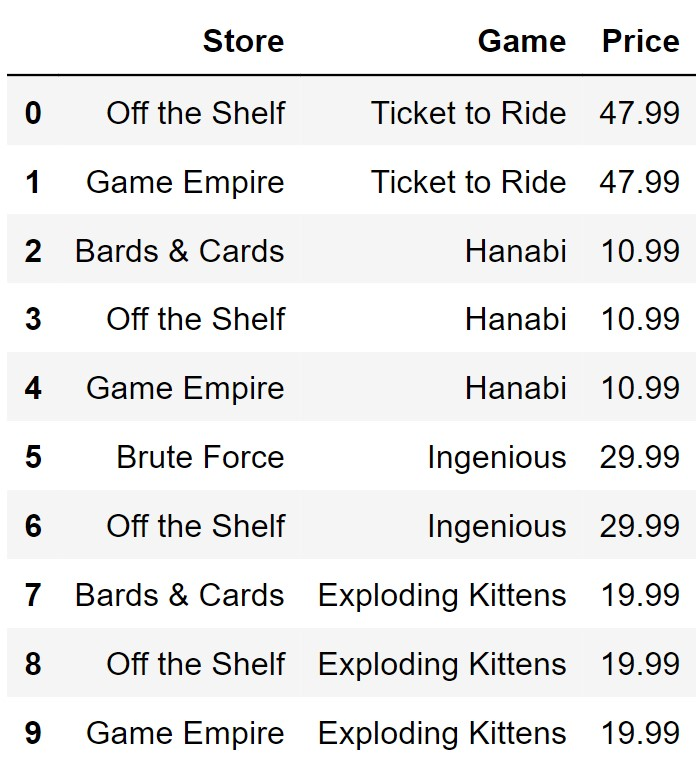
\includegraphics[width=2.5in]{final_images/merged.jpg}
\end{center}

\newpage

        In the space below, specify what the DataFrame \texttt{prices} \textbf{could} look like. The column labels should go in the top row, and the row labels (index) should go in the leftmost row. You may not need to use all the columns provided, but you are told that  \texttt{prices} has five rows, so you should use all rows provided.

        \vspace{0.1in}

         \textbf{Note:} There are several correct answers to this question.

\begin{center}
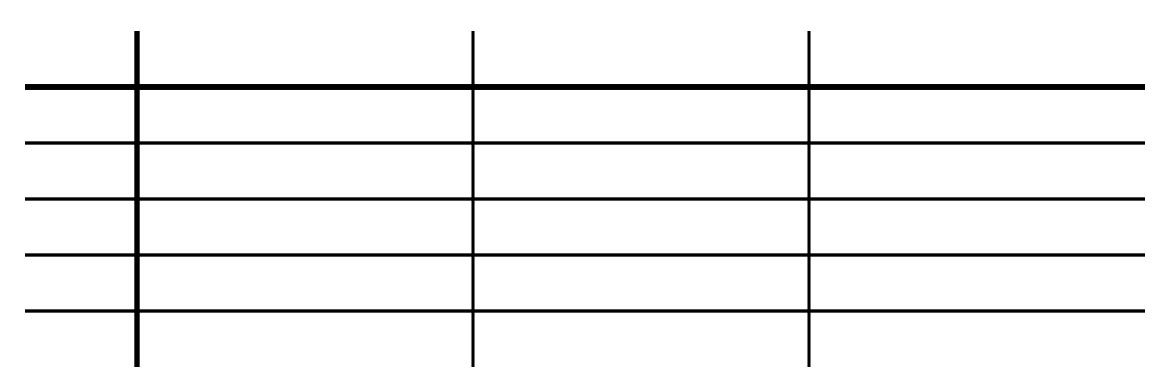
\includegraphics[width=6in]{final_images/blank_df.jpg}
\end{center}

# BEGIN SOLN


One solution is shown below.
\begin{center}
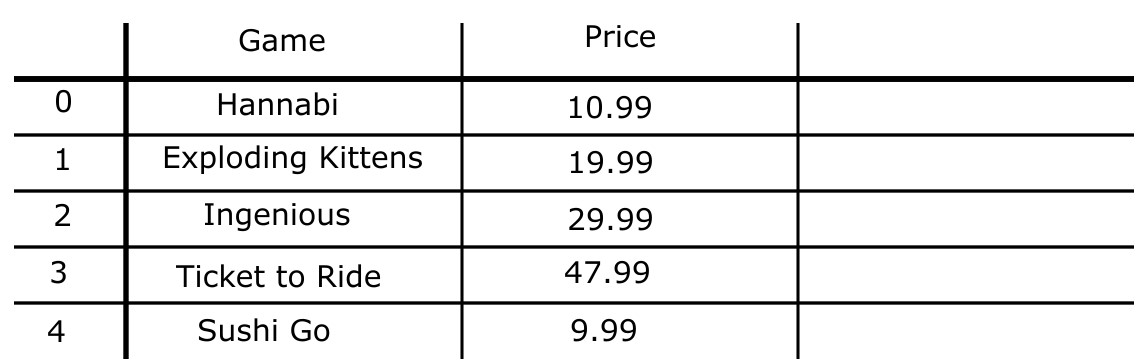
\includegraphics[width=5.9in]{final_images/filled_prices.jpg}
\end{center} 
A correct answer should have two columns, \texttt{"Game"} and \texttt{"Price"}. Four of the rows should be the ones shown here in the first four rows, and there should be one additional row, which can contain any game besides the ones already appearing in the first four rows, and any price. Any ordering of the rows and columns will be considered correct.


# END SOLN

    

# END SUBPROB
    # BEGIN SUBPROB


        Suppose \texttt{merged} now contains all the available games and their corresponding prices at each store (in particular, a given game is sold for the same price at all stores). You want to buy as many games as possible but you only want to go to one store. Which store should you go to maximize the number of games you can buy?

        Fill in the blanks so that \texttt{where\_to\_go} evaluates to the name of the store you should buy your games from.

\begin{verbatim}
where_to_go = (merged.groupby("Store").__(a)__
                     .sort_values(by="Price", ascending=False)
                     .__(b)__)
\end{verbatim}

    \begin{enumerate}[label=(\roman*)]
    \item What goes in blank (a)?

    \begin{center}
    ( ) \texttt{min()}    
    ( ) \texttt{max()}    
    ( ) \texttt{count()}    
    ( ) \texttt{mean()}  
    \end{center}

    \item What goes in blank (b)?  
    \inlineresponsebox[4in]{\texttt{index[0]}}
    \end{enumerate}
    

    

# END SUBPROB
    # BEGIN SUBPROB


        Suppose you go to the store \texttt{where\_to\_go} and buy one copy of each of the available games that you enjoyed at game night. How much money will you spend? Write one line of code that evaluates to the answer, using the \texttt{merged} DataFrame and no others.

        \begin{responsebox}{1in}
            \texttt{merged[merged.get("Store")==where\_to\_go].get("Price").sum()}
        \end{responsebox}
    

# END SUBPROB




# END PROB


\newpage
# BEGIN PROB

[(12 pts)]

We collect data on the play times of 100 games of \textit{Chutes and Ladders} (sometimes known as \textit{Snakes and Ladders}) and want to use this data to perform a hypothesis test. 


    # BEGIN SUBPROB


        Which of the following pairs of hypotheses can we test using this data?

        \vspace{0.1in}

        ( ) \textbf{Null Hypothesis}: In a random sample of \textit{Chutes and Ladders games, the average \\
        \hspace*{1em}\phantom{\textbf{Null Hypothesis: }} play time is 30 minutes.\\
        \hspace*{1em}\textbf{Alternative Hypothesis}: In a random sample of \textit{Chutes and Ladders} games, the \\
        \hspace*{1em}\phantom{\textbf{Alternative Hypothesis: }}average play time is not 30 minutes.}

        \vspace{0.1in}

        ( ) \textbf{Null Hypothesis}: In a random sample of \textit{Chutes and Ladders games, the average \\
        \hspace*{1em}\phantom{\textbf{Null Hypothesis: }} play time is not 30 minutes.\\
        \hspace*{1em}\textbf{Alternative Hypothesis}: In a random sample of \textit{Chutes and Ladders} games, the \\
        \hspace*{1em}\phantom{\textbf{Alternative Hypothesis: }}average play time is 30 minutes.}

        \vspace{0.1in}

        ( ) \textbf{Null Hypothesis}: A game of \textit{Chutes and Ladders takes, on average, 30 minutes \\
        \hspace*{1em}\phantom{\textbf{Null Hypothesis: }}to play.\\
        \hspace*{1em}\textbf{Alternative Hypothesis}: A game of \textit{Chutes and Ladders} does not take, on average,\\
        \hspace*{1em}\phantom{\textbf{Alternative Hypothesis: }}30 minutes to play.}

        \vspace{0.1in}

        ( ) \textbf{Null Hypothesis}: A game of \textit{Chutes and Ladders does not take, on average, 30 \\
        \hspace*{1em}\phantom{\textbf{Null Hypothesis: }}minutes to play.\\
        \hspace*{1em}\textbf{Alternative Hypothesis}: A game of \textit{Chutes and Ladders} takes, on average, 30\\
        \hspace*{1em}\phantom{\textbf{Alternative Hypothesis: }}minutes to play.}
        
    

# END SUBPROB
    # BEGIN SUBPROB


        We use our collected data to construct a 95\% CLT-based confidence interval for the average play time of a game of \textit{Chutes and Ladders}. This 95\% confidence interval is $[26.47, 28.47]$. For the 100 games for which we collected data, what is the mean and standard deviation of the play times?

        \begin{center}
        mean = \inlineresponsebox[1in]{27.47}, SD = \inlineresponsebox[1in]{5}
        \end{center}

    

# END SUBPROB
    # BEGIN SUBPROB


        Does the CLT say that the distribution of play times of the 100 games is roughly normal?

        \begin{center}
            ( ) Yes}   \hspace{1in     
            ( ) No        
        \end{center}
        
    

# END SUBPROB
    # BEGIN SUBPROB


        Of the two hypotheses you selected in part (a), which one is better supported by the data?

        \begin{center}
            ( ) Null Hypothesis        
            ( ) Alternative Hypothesis        
        \end{center}
        
    

# END SUBPROB




# END PROB

\newpage

Feel free to draw us a picture or tell us about your fondest memory from DSC 10 this
quarter.

\begin{responsebox}{7.5in}
My favorite memory was feeling proud after making this picture:

\begin{center}
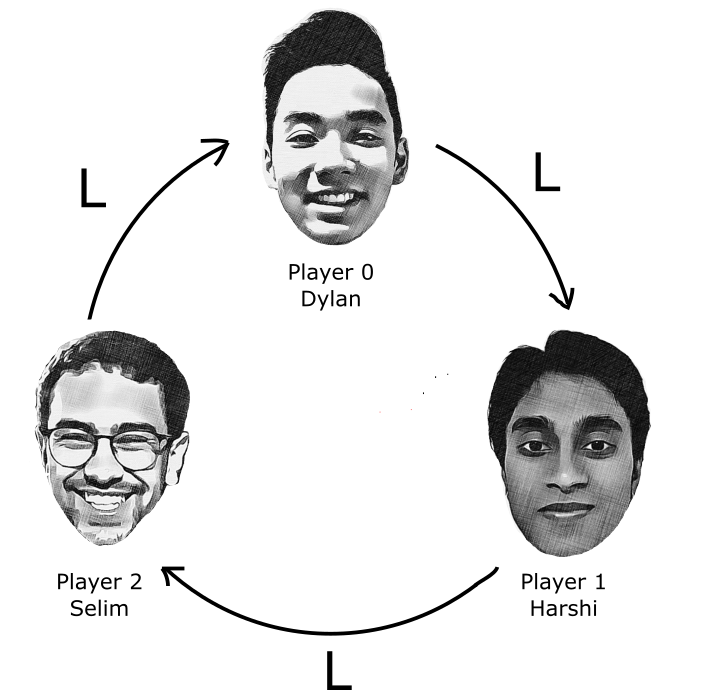
\includegraphics[width=6in]{final_images/lcr.png}
\end{center}

This quarter I also had some of my most memorable office hours interactions, such as when one student demonstrated several mathemagical tricks, and when another told me he tried to read my dissertation!

I also had a great time at our staff dinner at Star Anise, and I had fun making mango sticky rice for our staff meeting!
\end{responsebox}

\textbf{Before turning in your exam, please make sure that your PID is on every page.}

\bigskip

\textbf{Congratulations on finishing DSC 10!}



\end{document}

% to do:
% add more questions
% add solutions for 5, 6, 7, 12, 14
% points
% versions



